\documentclass[11pt]{article}

% Paquetes
%===============================================================================

% Paquete para incluir imagenes
\usepackage{graphicx}
\graphicspath{ {./images/} }

% Paquete para incluir trozos de codigo
\usepackage{listings, listings-rust}

% Para que el codigo acepte caracteres en utf8
\lstset{literate=
  {á}{{\'a}}1 {é}{{\'e}}1 {í}{{\'i}}1 {ó}{{\'o}}1 {ú}{{\'u}}1
  {Á}{{\'A}}1 {É}{{\'E}}1 {Í}{{\'I}}1 {Ó}{{\'O}}1 {Ú}{{\'U}}1
  {à}{{\`a}}1 {è}{{\`e}}1 {ì}{{\`i}}1 {ò}{{\`o}}1 {ù}{{\`u}}1
  {À}{{\`A}}1 {È}{{\'E}}1 {Ì}{{\`I}}1 {Ò}{{\`O}}1 {Ù}{{\`U}}1
  {ä}{{\"a}}1 {ë}{{\"e}}1 {ï}{{\"i}}1 {ö}{{\"o}}1 {ü}{{\"u}}1
  {Ä}{{\"A}}1 {Ë}{{\"E}}1 {Ï}{{\"I}}1 {Ö}{{\"O}}1 {Ü}{{\"U}}1
  {â}{{\^a}}1 {ê}{{\^e}}1 {î}{{\^i}}1 {ô}{{\^o}}1 {û}{{\^u}}1
  {Â}{{\^A}}1 {Ê}{{\^E}}1 {Î}{{\^I}}1 {Ô}{{\^O}}1 {Û}{{\^U}}1
  {ã}{{\~a}}1 {ẽ}{{\~e}}1 {ĩ}{{\~i}}1 {õ}{{\~o}}1 {ũ}{{\~u}}1
  {Ã}{{\~A}}1 {Ẽ}{{\~E}}1 {Ĩ}{{\~I}}1 {Õ}{{\~O}}1 {Ũ}{{\~U}}1
  {œ}{{\oe}}1 {Œ}{{\OE}}1 {æ}{{\ae}}1 {Æ}{{\AE}}1 {ß}{{\ss}}1
  {ű}{{\H{u}}}1 {Ű}{{\H{U}}}1 {ő}{{\H{o}}}1 {Ő}{{\H{O}}}1
  {ç}{{\c c}}1 {Ç}{{\c C}}1 {ø}{{\o}}1 {å}{{\r a}}1 {Å}{{\r A}}1
  {€}{{\euro}}1 {£}{{\pounds}}1 {«}{{\guillemotleft}}1
  {»}{{\guillemotright}}1 {ñ}{{\~n}}1 {Ñ}{{\~N}}1 {¿}{{?`}}1 {¡}{{!`}}1
}

% Para que los metadatos que escribe latex esten en español
\usepackage[spanish]{babel}

% Para la bibliografia
% Sin esto, los enlaces de la bibliografia dan un error de compilacion
\usepackage{url}

% Metadatos del documento
%===============================================================================
\title{
    {Práctica 1b}\\
    {Técnicas de Búsqueda Local y Algoritmos Greedy}\\
    {Problema de Agrupamiento con Restricciones}\\
}
\author{
    {Sergio Quijano Rey - 72103503k}\\
    {4º Doble Grado Ingeniería Informática y Matemáticas}\\
    {Grupo de prácticas 2 - Viernes 17.30h a 19.30h}\\
    {sergioquijano@correo.ugr.es}
}
\date{\today}

% Separacion entre parrafos
\setlength{\parskip}{1em}

% Contenidos del documento
%===============================================================================

\begin{document}

% Portada del documento
\maketitle
\pagebreak

% Indice de contenidos
\tableofcontents
\pagebreak

% Primer ejercicio
\section{Descripción del problema}

Vamos a trabajar el problema del agrupamiento con restricciones (\textbf{\emph{PAR}}). Consiste en una generalización del problema de agrupamiento clásico, al que añadimos restricciones sobre los datos.

El problema de agrupamiento clásico consiste en, dados unos datos de entrada sin etiquetar $X$ de tamaño $n$, agruparlos en $k$ grupos (o en inglés, \emph{clusters}) diferentes, formando una partición $C$ de $X$, de forma que se optimice alguna métrica. Normalmente, se busca minimizar la distancia \emph{intra\_cluster} (que más tarde se definirá).

La diferencia con el problema de agrupamiento clásico, por tanto, es la inclusión de restricciones. En nuestro caso concreto, trabajemos con restricciones entre pares de puntos, que además serán de dos tipos:

\begin{itemize}
    \item Restricción tipo \emph{Must Link}: los dos puntos afectados por esta restricción deberán pertenecer al mismo cluster
    \item Restricción tipo \emph{Cannot Link}: los dos puntos afectados por esta restricción no deben pertenecer al mismo cluster
\end{itemize}

Consideraremos de forma débil estas restricciones, es decir, podemos incumplir algunas restricciones. Pero supondrá que la solución será de peor calidad. Para especificar mejor esta noción, definimos la función de \emph{fitness} que buscamos minimizar:

\begin{displaymath}
    fitness(sol) := distancia_{intra-cluster}(sol) + \lambda * infeasibility(sol)
\end{displaymath}

donde $infeasibility$ es el número de restricciones que se incumplen. Esta función de $fitness$ nos permite pasar de intentar optimizar dos funciones objetivo a solo tener que optimizar un objetivo. El valor de $\lambda$ se especifica más adelante.

Como los datos no están etiquetados a priori, podríamos considerar este problema como un problema de aprendizaje no supervisado. Sin embargo, se puede considerar que las restricciones nos dan un tipo de etiquetado, por lo que es más correcto pensar que estamos ante una tarea de aprendizaje \emph{semi-supervisado}. La principal utilidad de resolver estos problemas es que normalmente estamos reduciendo la dimensionalidad de los datos a analizar, y de este modo, es más sencillo extraer conocimiento sobre dichos datos. También es útil para realizar

\pagebreak

% TODO -- es un máximo de 4 páginas y esto ocupa 5 páginas
% TODO -- describir en pseudo la funcion objetivo y los operadores comunes? ==> Apartado d
\section{Descripción de la aplicación de los algoritmos empleados}

\subsection{Representación del conjunto de datos}

Los datos vienen dados en una matrix de tamaño $n x d$ donde $n$ es el número de puntos y $d$ es la dimensión de cada uno de los puntos.

\subsubsection{Representación del conjunto de datos en código}

El conjunto de datos viene representado en \lstinline{problem_datatypes::DataPoints} que contiene un vector de otro tipo de dato: \lstinline{problem_datatypes::Point}. El tipo de dato \lstinline{Point} tiene un campo que es de tipo \lstinline{ndarray::Array1<f64>} que representa un vector (usamos una librería para trabajar con matrices y vectores). Por tanto, hemos pasado de trabajar con una matriz de datos a trabajar con un vector de puntos. Esto nos permite trabajar de forma más expresiva y sencilla con el problema. Por ejemplo, podemos calcular con métodos del \lstinline{struct} distancia entre dos puntos, centroide de un conjunto de puntos, \ldots

\subsection{Representación de las restricciones}

Las restricciones vienen dadas en un fichero de datos que representa una matriz que codifica las restricciones de la siguiente forma:

\begin{itemize}
    \item El elemento en la fila $i$-ésima y columna $j$-ésima representa las restricciones que hay entre el punto $i$ y el punto $j$
    \item Como la restricción que tenga el punto $i$ con el punto $j$ implica que el punto $j$ tiene la misma restricción con el punto $i$, es claro que dicha matriz debe ser simétrica
    \item Un valor $0$ significa que no hay restricciones. Un valor $1$ significa que hay una restricción tipo \emph{Must Link}. Un valor $-1$ implica una restricción \emph{Cannot Link}
    \item Además, la matriz tiene la diagonal de $1$s
\end{itemize}

\subsubsection{Representación de las restricciones en código}

El \lstinline{struct} \lstinline{problem_datatypes::Constraints} junto al enumerado \lstinline{problem_datatypes::ConstraintType} representan en el código las restricciones. El código es el siguiente:

\begin{lstlisting}[language=Rust, style=Boxed]
pub enum ConstraintType {
    MustLink,
    CannotLink,
}

pub struct Constraints{
    data: HashMap<(i32, i32), ConstraintType>,
}
\end{lstlisting}

Es claro que guardamos pares de enteros, que marcan los índices de los puntos, y la restricción entre el par de puntos representados, en un \lstinline{HashMap}. Esta elección viene motivada por:

\begin{itemize}
    \item Podemos acceder a las restricciones entre dos puntos en tiempo constante
    \item Podemos iterar sobre todas las restricciones, gracias a los métodos proporcionados por el lenguaje de programación, en un tiempo más que razonable. Así iteramos solo sobre una lista de $r$ restricciones, en vez de sobre una matriz cuadrada de dimensión $n^2$
    \item En cierto modo, estamos combinando los beneficios de tener acceso directo a elementos concretos y los beneficios de poder iterar sobre una lista (aunque iterar sobre un \lstinline{Hash} puede ser algo más lento que iterar sobre una lista o un \lstinline{array})
    \item Es fácil de implementar métodos para operar con restricciones con este tipo de dato
\end{itemize}

La implementación de los métodos que permiten manipular el \lstinline{struct} aseguran que:
\begin{itemize}
    \item No guardamos la restricción $(i, j)$ y junto a la $(j, i)$. Solo guardamos una de las dos restricciones, ahorrando memoria
    \item De hecho, el criterio es guardar como índices el par $(i, j)$ donde $i \leq j$
    \item Tampoco guardamos las restricciones $(i, i), MustLink$ pues son restricciones triviales
\end{itemize}


\subsection{Representación de la solución}

Una representación de la solución será un vector de tamaño $n$ con valores en $\{0, \ldots, k - 1\}$ donde $n$ es el número de puntos y $k$ es el número de clusters en los que dividimos los datos. Este vector representa la partición de los datos en los $k$ clusters. En la posición $i$-ésima del vector, guardamos el cluster al que pertenece el punto $i$-ésimo de nuestro conjunto de datos.

Las soluciones deben cumplir las siguientes restricciones:

\begin{itemize}
    \item No pueden quedar clusters vacíos. Es decir, clusters a los que no haya ningún punto asignado. Esto puede verse viendo que $\forall i \in \{0, \ldots, k-1\}$ $\exists pos \in \{0, \ldots, n-1\}$ tal que $solution[pos] = i$, es decir, el vector de soluciones tiene al menos una vez cada valor posible de los clusters
    \item Cada punto solo puede pertenecer a un único cluster. Por la forma vectorial en la que representamos la partición, esta restricción se verifica forzosamente, y por tanto no nos tenemos que preocupar de realizar comprobaciones
    \item La unión de los puntos de los clusters debe ser todo el conjunto de datos, es decir, $X = \bigcup c_i$. De nuevo, nuestra representación vectorial fuerza a que esta restricción se verifique
\end{itemize}

Por ejemplo, si tenemos 5 puntos y 3 clusters, una posible solución sería $\{3, 1, 2, 3, 0\}$. Y por otro lado, la solución $\{3, 1, 2, 3, 2\}$ no es válida pues el cluster $0$ está vacío.

Para cada solución podemos calcular algunas métricas necesarias para conocer el valor de $fitness$ de la solución que estamos representando. Para comenzar, por cada cluster podemos calcular el \textbf{centroide} del cluster:

\begin{displaymath}
    \vec{\mu_i} := \frac{1}{|c_i|} \sum_{x_i \in c_i} \vec{x_i}
\end{displaymath}

Definimos para cada cluster su \textbf{distancia media intra-cluster} como:

\begin{displaymath}
    \bar{c_i} := \frac{1}{|c_i|} \sum_{x_i \in c_i} || \vec{x_i} - \vec{\mu_i} ||_2
\end{displaymath}

Y con ello podemos definir la \textbf{desviación general de la partición} como:

\begin{displaymath}
    \bar{c} := \frac{1}{k} \sum_{i \in 1, \ldots k} \bar{c_i}
\end{displaymath}

Definimos $infeasibility$ como el número de restricciones, tanto del tipo \emph{Must Link} como del tipo \emph{Cannot Link}, que se violan.

Con ello, ya podemos definir el valor de $\lambda$ como $\lambda := \frac{D}{|R|}$ donde $|R|$ es el número total de restricciones y $D$ la distancia máxima entre dos puntos de $X$.


\subsubsection{Representación de la solución en código}

La solución se representa en la clase \lstinline{problem_datatypes::Solution}. El código de los campos del \lstinline{struct} desarrollado es:

\begin{lstlisting}[language=Rust, style=Boxed]
pub struct Solution<'a, 'b> {
    cluster_indexes: Vec<u32>,
    data_points: &'a DataPoints,
    constraints: &'b Constraints,
    number_of_clusters: i32,

    /// Representa el peso de infeasibility en el calculo de fitness
    /// Solo se calcula una vez al invocar a Solution::new
    lambda: f64,

    // Para cachear el valor de fitness pues es un calculo costoso de realizar
    // Como los datos del struct no cambian, podemos hacer el cacheo sin miedo
    // Usamos RefCell para tener un patron de mutabilidad interior
    fitness: RefCell<Option<f64>>,
}
\end{lstlisting}

Los campos del \lstinline{struct} representan:

\begin{itemize}
    \item \lstinline{cluster_indixes}: el vector solución que representa la asignación de puntos a clusters
    \item \lstinline{data_points}: referencia al conjunto de datos (sirve para calcular métricas como el $fitness$ de la solución que se representa)
    \item \lstinline{constraints}: referencia al conjunto de restricciones sobre los datos (sirve para calcular métricas como el $fitness$ de la solución que se representa)
    \item \lstinline{number_of_clusters}: número de clusters en los que se agrupan los datos (sirve para comprobar que una solución sea válida)
    \item \lstinline{lambda}: valor de $\lambda$, necesario para calcular el $fitness$
    \item \lstinline{fitness}: valor de $fitness$. Está incluida en un \lstinline{RefCell<Option<f64>>} para poder cachear su valor, puesto que los atributos de una instancia nunca cambian y el cálculo del valor $\lambda$ es muy costoso (implica calcular restricciones violadas y distancias entre puntos)
\end{itemize}

La comprobación de que no tenemos clusters sin puntos asignados se hace en el método \lstinline{Solution::is_valid}. La distancia media intracluster se calcula en \lstinline{Solution::intra_cluster_distance}. Mientras que la desviación general se calcula en \lstinline{Solution::global_cluster_mean_distance}. El valor de $infeasibility$ se calcula en \lstinline{Solution::infeasibility}. El cálculo de $\lambda$ se realiza en el \emph{constructor} del \lstinline{struct}.

\pagebreak

\section{Descripción de los algoritmos empleados}

\subsection{Búsqueda Local}

Usamos un pseudocódigo muy parecido a \lstinline{Python} pues es muy expresivo y facilita traducir partes de nuestro código real a pseudocódigo.

Método de exploración de entorno:

\begin{lstlisting}[language=Python, style=Boxed]
# Estrategia el primero mejor
# Devuelve el primer vecino que mejora la solucion actual
def get_neighbour():
    # Tomamos el generador de vecinos que se describe mas adelante
    neighbours_generator = generate_all_neighbours()

    # Mezclo los generadores de vecinos
    neighbours_generator.shuffle()

    # Exploro los vecinos hasta encontrar uno mejor que esta solucion
    for current_generator in neighbours_generator:
        current_solution = self.generate_solution_from(current_generator)

        if
            current_solution.is_valid() &&
            current_solution.fitness() < self.fitness():

            return current_solution

    # No hemos encontrado un vecino mejor
    return None;
}
\end{lstlisting}

Operador de generación de vecino:

\begin{lstlisting}[language=Python, style=Boxed]

# Struct que representa el generador de vecinos de
# forma eficiente
struct NeighbourGenerator:
    # El elemento que queremos mover de cluster
    element_index: i32,

    # El nuevo cluster al que asignamos el elemento
    new_cluster: u32,

# Funcion que genera todos los vecinos posibles de un elemento
# Los vecinos generados pueden ser no validos
def generate_all_neighbours(
    number_of_elements,
    number_of_clusters):
    neighbours = []

    for current_element in 0..number_of_elements:
        for current_cluster in 0..number_of_clusters:
            neighbours.append(NeighbourGenerator{
                current_element,
                current_cluster,
            });

    return neighbours;
\end{lstlisting}

Generación de soluciones aleatorias:

\begin{lstlisting}[language=Python, style=Boxed]
# Genera una solucion inicial aleatoria como punto de partida de las busquedas
# Puede dejar clusters vacios, por lo que el caller de esta funcion tiene que
# comprobar la validez de la solucion aleatoria, y en caso de invalidez, volver
# a llamar a esta funcion (es muy poco probable que con muchos puntos dejemos
# un cluster vacio)
def generate_random_solution(data_points, constraints, number_of_clusters):
    # Vector con indices de clusters aleatorios, de tamaño el numero de puntos
    # que trabajamos
    random_cluster_indixes = [
        random(0, number_of_clusters)
        for _ in data_points.len()
    ]

    # En nuestro codigo, generamos el struct Solution a partir de los parametros
    # de entrada y random_cluster_indixes
    return solution_from(cluster_indexes)
}
\end{lstlisting}


\pagebreak

% TODO -- no se indica maximo pero por el apartado anterior pareciese razonable que fuesen solo dos paginas
% TODO -- creo que solo hay que poner pseudocodigo
\section{Descripción y Pseudocódigo de los algoritmos de comparación}

Como algoritmo de comparación estamos considerando una modificación del algoritmo clásico \emph{K-means} al que añadimos la capacidad de considerar las restricciones: \emph{copkmeans} o \emph{Constrained K-means}. Por tanto, estamos ante un algoritmo \emph{greedy}.

La idea general es:

\begin{enumerate}
    \item Partir de una solución inicial aleatoria, que vendrá dada por una asignación de centroides de clusters aleatorios
    \item Iterar sobre todos los datos en orden aleatorio, asignando a cada punto el mejor cluster en ese momento (siguiendo claramente un esquema greedy). Consideramos como mejor cluster el que menos restricciones violadas produzca, y en caso de empate, el cluster cuyo centroide sea más cercano al punto
    \item Una vez acabada la asignación de todos los puntos, calcular los centroides de los clusters con la asignación actual de los puntos
    \item Repetir el proceso desde 2 si los centroides han cambiado respecto de la anterior iteración
\end{enumerate}

A la hora de ejecutar el algoritmo, en algunos \emph{datasets} daba problemas, pues los centroides oscilaban infinitamente entre dos soluciones muy cercanas (debido entre otros factores a la configuración de los datos de entrada). Esta configuración de los datos también puede provocar que haya clusters que se queden sin puntos asignados, generando así una solución no válida. Por tanto, el algoritmo admite un parámetro de entrada para indicar si queremos que sea \emph{robusto} o no. En caso de que indiquemos que queremos que sea robusto se tendrán las siguientes diferencias:

\begin{itemize}
    \item Los centroides aleatorios no se tomarán como puntos aleatorios, sino como puntos del \emph{dataset} aleatorios, por lo que en una primera iteración no podrán quedar clusters vacíos, aunque si podrán quedar clusters vacíos en iteraciones posteriores. Con esto se buscas evitar el problema de los clusters vacíos
    \item Se tendrá un máximo de iteraciones. Este máximo lo hemos establecido como 50 iteraciones sobre el bucle principal. Teniendo en cuenta que cuando no cicla infinitamente, en menos de 10 iteraciones el algoritmo encuentra solución, consideramos que es un máximo mucho más que aceptable para asegurar que la solución devuelta sea la mejor (o la segunda mejor) que el \emph{greedy} puede calcular con esa semilla aleatoria. Con esto se busca evitar el problema del ciclado infinito
    \item Aún con estos cambios, en ciertas ocasiones no podemos evitar que dejemos un cluster vacío en iteraciones posteriores a la primera. Por tanto, también colocaremos un máximo de reinicios del algoritmo en la parte del código que llama al método de búsqueda.
\end{itemize}

Aún con estos cambios, en ciertas ocasiones no podemos evitar que dejemos un cluster vacío en iteraciones posteriores a la primera. Esto lo comentaremos más en profundidad en el análisis de los resultados

El pseudocódigo (en notación muy parecida a \lstinline{Python}) de nuestra implementación del algoritmo quedaría tal que:

\begin{lstlisting}[language=Python, style=Boxed]
# Generamos los centroides aleatorios. Dependiendo de si es robust o no
# consideramos puntos aleatorios en [0,1] x [0,1] o puntos del dataset
# de entrada aleatorios
current_centroids = generate_random_centroids()

# Solucion inicial aleatoria que se va a modificar en la primera iteracion
# Notar que no es valida porque deja todos los clusters menos uno vacíos
current_cluster_indixes = [0, 0, ..., 0]

# Para comprobar que los centroides cambien
centroids_have_changed = true


# Si robust == true, acotamos el numero maximo de iteraciones
max_iterations = 50
mut curr_iteration = 0

while centroids_have_changed == true and curr_iteration < max_iterations{

    # Realizamos una nueva asignacion de clusters. Recorremos los puntos
    # aleatoriamente y asignamos el cluster que menos restricciones viole
    # en esa iteracion. En caso de empate, se toma el cluster con centroide
    # mas cercano al punto
    new_cluster_indixes = assign_points_to_clusters()

    # Comprobamos que la nueva solucion calculada es correcta
    if valid_cluster_configuration(current_cluster_indixes) == false:
        # Esto hace que el el caller de la funcion copkmeans, se muestre un
        # mensaje por pantalla y se vuelva a realizar la busqueda, con lo que
        # partimos de unos centroides aleatorios nuevos. Como ya se ha comentado,
        # hay un maximo de reinicios en el caller para este metodo
        return None

    # Calculamos los nuevos centroides y comprobamos si han cambiado
    new_centroids = calculate_new_centroids(new_cluster_indixes)
    centroids_have_changed = centroids_are_different(
        current_centroids,
        new_centroids
    )

    # Cambiamos a la nueva asignacion de clusters y los nuevos centroides
    current_cluster_indixes = new_cluster_indixes
    current_centroids = new_centroids


    # En caso de que robust = true, acotamos el numero de iteraciones de forma
    # efectiva aumentando el contador. En otro caso, al no tocar el contador
    # no estamos teniendo en cuenta este parametro
    if robust == true:
        curr_iteration = curr_iteration + 1;

# Devolvemos la solucion en la estructura de datos correspondiente
return solution_from(current_cluster_indixes)
\end{lstlisting}

Desarrollamos el código de \lstinline{assign_points_to_clusters} por su importancia:

\begin{lstlisting}[language=Python, style=Boxed]
def assign_points_to_clusters():
    # Realizamos una nueva asignacion de clusters
    # -1 para saber que puntos todavia no han sido asignados a un cluster
    new_cluster_indixes= [-1, -1, ..., -1]

    # Recorremos aleatoriamente los puntos para irlos asignando a cada cluster
    point_indexes = (0..data_points.len())
    point_indexes.shuffle();

    for index in point_indexes:
        # Calculo el cluster al que asignamos el punto actual
        new_cluster_indixes[index] = select_best_cluster(
            current_cluster_indixes,
            current_centroids,
        )

    # Devolvemos los indices que representan la solucion
    return new_cluster_indixes
\end{lstlisting}

\pagebreak

\section{Explicación del procedimiento considerado para desarrollar la práctica}

Hemos desarrollado todo el código desde prácticamente cero usando el lenguaje de programación \lstinline{Rust}. Para el entorno de desarrollo, solo hace falta instalar \lstinline{Cargo} que permite compilar el proyecto, correr los ejecutables cómodamente, descargar las dependencias o correr los tests que se han desarrollado.

Las librerías externas que hemos empleado pueden consultarse en el fichero \lstinline{Cargo.toml} en el que se incluye un pequeño comentario sobre la utilidad de cada librería.

A continuación describimos el proceso de instalación y un pequeño manual de usuario para compilar y ejecutar el proyecto en \lstinline{Linux} (pues es el sistema operativo que nuestro profesor de prácticas, Daniel Molina, nos ha indicado que usa).

\subsection{Instalación del entorno}

Lo más sencillo y directo es instalar \lstinline{rustup} \footnotemark que se encargará de instalar todos los elementos necesarios para compilar y ejecutar la práctica. Para ello podemos ejecutar:

\begin{itemize}
    \item En cualquier distribución linux: \lstinline{curl --proto '=https' --tlsv1.2 -sSf https://sh.rustup.rs | sh} y seguir las instrucciones
    \item Por si acaso no tenemos actualizado el entorno: \lstinline{rustup update}
\end{itemize}

Una vez tengamos instalado \lstinline{rustup}, podemos ejecutar órdenes como \lstinline{cargo check}, \lstinline{rustc}, \ldots

\footnotetext{Información actualizada sobre el proceso de instalación puede consultarse en \cite{Gettings40:online}, \cite{InstallR15:online} o \cite{rustuprs85:online}}

\subsection{Compilación y ejecución del binario}

Además del binario aportado en la estructura de directios que se especifica en el guión, podemos generar fácilmente el binario con \lstinline{cargo} y ejecutarlo tal que:

\begin{itemize}
    \item Para compilar: \lstinline{cargo build --release} lo que nos generará un binario en \lstinline{./target/release/PracticasMetaheuristicas}
    \item Podemos usar ese binario para ejecutar el programa o podemos usar \lstinline{cargo run --release <parametros entrada>} para correr el programa de forma más cómoda
    \item Es muy importante la opción \lstinline{--release} porque de otra forma el binario no será apenas optimizado, lo que supondrá tiempos de ejecución mucho mayores
    \item Para correr los tests programados podemos hacer \lstinline{cargo test}
\end{itemize}

Si ejecutamos el binario sin parámetros, veremos por pantalla un mensaje indicando los parámetros que debemos pasar al programa. Estos parámetros son:

\begin{itemize}
    \item fichero de datos: el fichero donde guardamos las coordenadas de los puntos
    \item fichero de restricciones
    \item Semilla para la generación de números aleatorios
    \item Número de clusters en los que queremos clasificar los datos
    \item Tipo de búsqueda: para especificar el tipo de algoritmo que queremos ejecutar. Los posibles valores son:
    \begin{itemize}
        \item copkmeans: búsqueda greedy
        \item copkmeans\_robust: búsqueda greedy con los cambios ya indicados para que sea algo más robusto
        \item local\_search: búsqueda local
    \end{itemize}
\end{itemize}

\subsection{Compilación y ejecución usando el script}

El proceso de compilación y ejecución del programa, sobre los distintos conjuntos de datos y restricciones, usando las distintas semillas que más adelante se especifican, se puede lanzar de forma cómoda invocando el script \lstinline{./launch_all_programs}.

\pagebreak

\section{Experimentos y análisis realizados}

\subsection{Descripción de los casos del problema empleados}

Para los cinco \textbf{valores de las semillas}, hemos elegido los siguientes: 123456789, 234567891, 3456789, 456789123 y 567891234 sin ningún criterio en concreto (podríamos haber buscado, por ejemplo, semillas que no diesen problemas a la hora de lanzar el algoritmo greedy).

Tenemos tres problemas distintos. Cada problema, tiene dos ficheros de restricciones, uno con el 10\% de los datos con restricciones, y otro con el 20\% de los datos con restricciones. Los problemas son:

\begin{itemize}
    \item Zoo: problema de agrupación de animales. Debemos clasificar datos de 16 dimensiones (o atributos) en 7 clusters distintos. Hay 101 instancias o puntos.
    \item Glass: problema de agrupación de vidrios. Debemos clasificar datos de 9 dimensiones en 7 clusters. Hay 214 instancias de datos
    \item Bupa: agrupar personas en función de hábitos de consumo de alcohol. Datos de dimensión 9 agrupados en 16 clusters. Hay 345 instancias de datos
\end{itemize}

Por tanto, haciendo cuentas, tenemos $3 * 2 * 5 = 30$ ejecuciones de búsquedas. De nuevo, estas 30 ejecuciones se pueden lanzar cómodamente usando \lstinline{./launch_all_programs}

Otros parámetros que hemos introducido en el programa son:

\begin{itemize}
    \item Máximo de iteraciones de la búsqueda local: 100.000
    \item Máximo de iteraciones del algoritmo greedy cuando forzamos la robustez: 50
    \item Máximo de repeticiones del algoritmo greedy cuando este deja clusters vacíos: 100
\end{itemize}

\pagebreak

\subsection{Resultados obtenidos según el formato especificado}

El formato especificado viene dado en una tabla de excel que hemos rellenado con los resultados mostrados por pantalla por el programa. Para obtener estos resultados, basta con lanzar \lstinline{./launch_all_programs > salida_datos.txt} y consultar el fichero creado. Ese fichero se entrega con la práctica para que pueda consultarse los datos con los que hemos generado las tablas.

\subsubsection{Resultados Greedy}

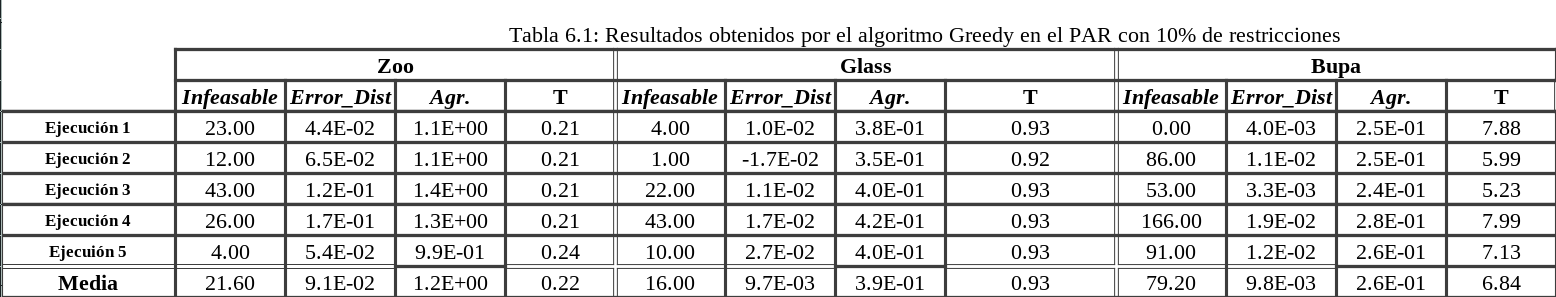
\includegraphics[width=\textwidth]{greedy_10}

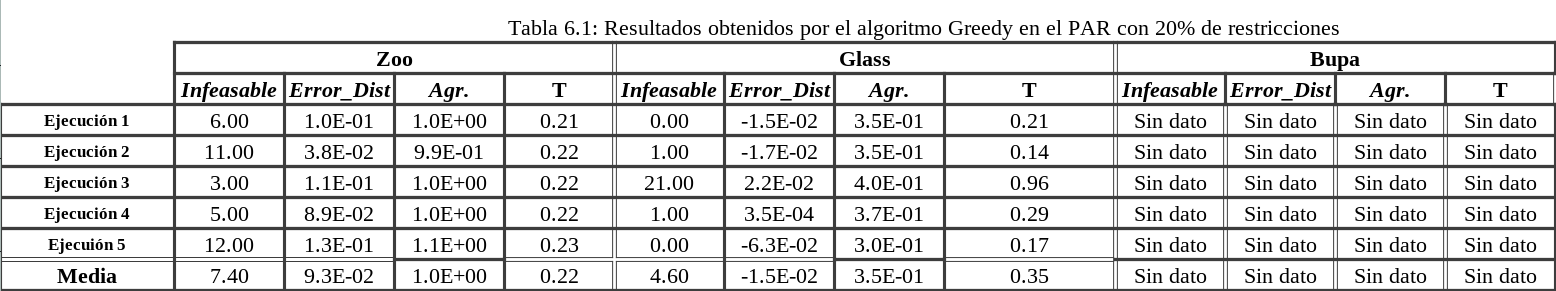
\includegraphics[width=\textwidth]{greedy_20}

\subsubsection{Resultados Búsqueda local}

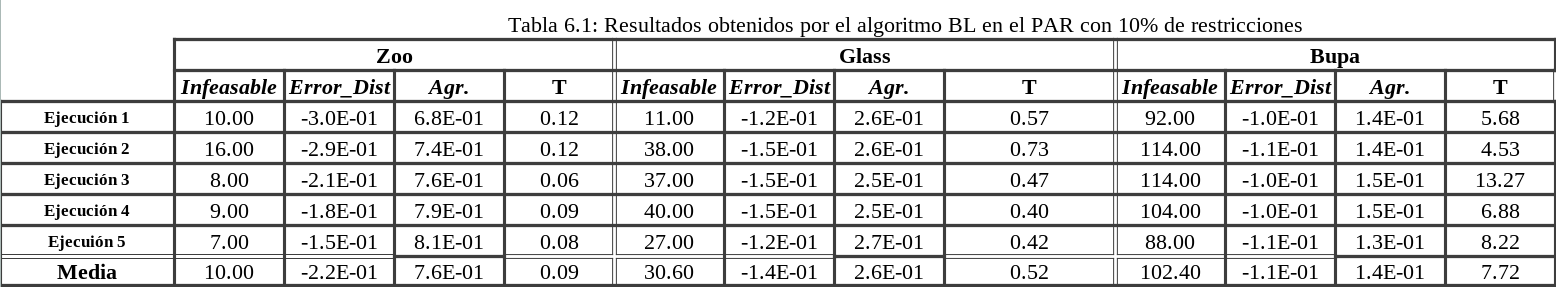
\includegraphics[width=\textwidth]{local_search_10}

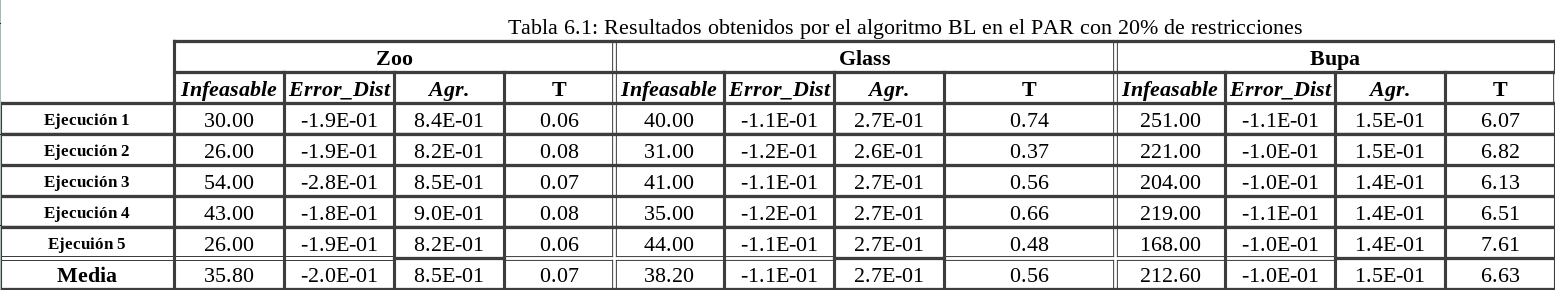
\includegraphics[width=\textwidth]{local_search_20}

\subsubsection{Comparación de resultados}

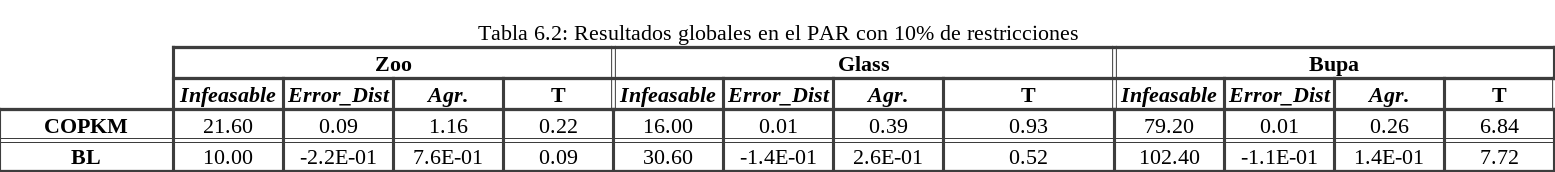
\includegraphics[width=\textwidth]{compare_10}

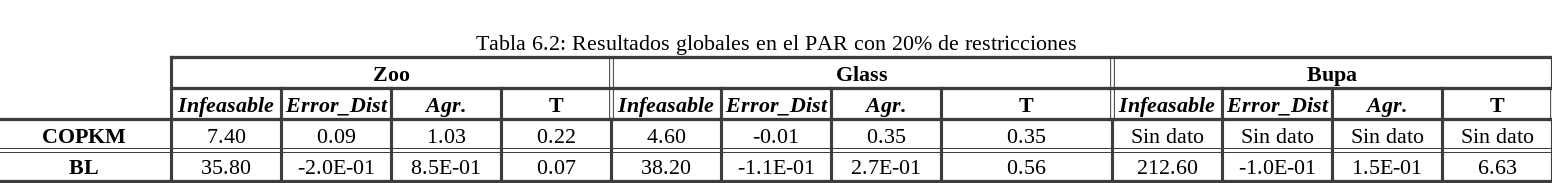
\includegraphics[width=\textwidth]{compare_20}

\subsection{Análisis de resultados}

Las comparaciones más directas se pueden hacer con las dos últimas tablas en las que comparamos valores medios. Lo primero que notamos es que el algoritmo greedy, sobre el \emph{dataset} de \emph{Bupa} con el 20\% de los datos, no ha sido capaz de encontrar solución con ninguna de las semillas. Es decir, en todos los casos ha necesitado más de 100 repeticiones del algoritmo desde cero. Podríamos haber decidido devolver la última solución válida obtenida en todos los procesos, pero esto prácticamente es lo mismo que devolver una solución aleatoria que sea válida. Por tanto, consideramos que es más representativo dejar la marca de que el algoritmo no ha conseguido obtener una solución.

En segundo lugar, es de esperar que el algoritmo greedy sea más rápido que el de búsqueda local. Sin embargo hay conjuntos de datos y restricciones en los que esto no pasa (por ejemplo, Zoo con 10\% y 20\% y Glass al 10\%). Esto puede deberse a que la búsqueda local caiga demasiado rápido en un óptimo local a partir de la solución aleatoria de partida. También influye que estemos usando la versión robusta del algoritmo greedy en la que acotamos por 50 iteraciones, pudiendo haber probado una cota menor a vista de las iteraciones requerridas en otros casos del problema en los que greedy converge sin ayudas.

En tercer lugar, también cabe esperar que greedy produzca soluciones con menores violaciones de restricciones, pues es el primer criterio voraz que estamos considerando (y en caso de empate según violaciones incumplidas, ya se considera el cluster más cercano). Esto se cumple en todos los \emph{datasets} salvo en Zoo al 10\%. Puede ser que al ser un espacio de búsqueda más pequeño, la búsqueda local consiga encontrar un buen óptimo que respete muchas más restricciones manteniendo una buena desviación general de la partición.

Además, es claro que la búsqueda local genera soluciones cuya desviación general de cluster está por debajo de los valores de referencia. Esto gracias a que estamos considerando a la vez en la función de fitness el número de restricciones violadas (ponderado por el valor de $\lambda$) y la desviación general del cluster. Del mismo modo, estamos obteniendo mejores valores del fitness en prácticamente todos los casos. Esto era de esperar pues en búsqueda local estamos optimizando este valor mientras que en el algoritmo greedy estamos simplemente siguiendo una estrategia voraz que pensamos que puede producir buenos resultados. Cuando no ocurre esto, podríamos pensar que el algoritmo greedy ha obtenido una muy buena solución por casualidad, o lo que parece más probable, que nuestra búsqueda local cae en un mal óptimo local en contadas ocasiones.

Pasamos ahora a comentar las tablas generales, no solo las de comparaciones. Podríamos hacer comentarios sobre el comportamiento del algoritmo greedy, como por ejemplo, su dependencia de la semilla inicial a la hora de obtener buenos o malos resultados, pero al ser un algoritmo de comparación base, no parece relevante que hagamos un profundo estudio sobre su comportamiento.

El valor del fitness se ve afectado por la semilla inicial (que determina la solución inicial de la que partimos) se ve afectado por la semilla inicial, pero no hay variaciones demasiado bruscas (como si ocurre, por ejemplo, en el greedy con los Zoo de 10\% y 20\% de restricciones). Sin embargo, si que podemos observar una variabilidad mucho más grande en la cantidad de restricciones violadas. En zoo 10\% podemos pasar de 7 violaciones a 16 (más del doble). En zoo 20\% podemos pasar de 26 a 54 (de nuevo, un poco más del doble). En bupa 20\%, podemos pasar de 168 a 251. Por tanto podemos pensar que es esta métrica es más sensible a la aleatoriedad que el fitness (en el que esta métrica compone el primer sumando de forma ponderada). Por ejemplo, para Zoo 10\%, las restricciones violadas tienen un
3.54 de desviación típica, mientras que el fitness tiene un 0.05 de desviación típica.

\subsubsection{Gráficas de evolución de fitness}

Estas gráficas han sido generadas a partir de la salida del programa y un script de \lstinline{Python} que emplea la librería \lstinline{matplotlib} para la generación de las gráficas. El código de generación de las gráficas se puede consultar en el fichero \lstinline{graficas.py}.

Podemos mirar las gráficas de evolución del error (o gráficas de convergencia) para Zoo 10\%:

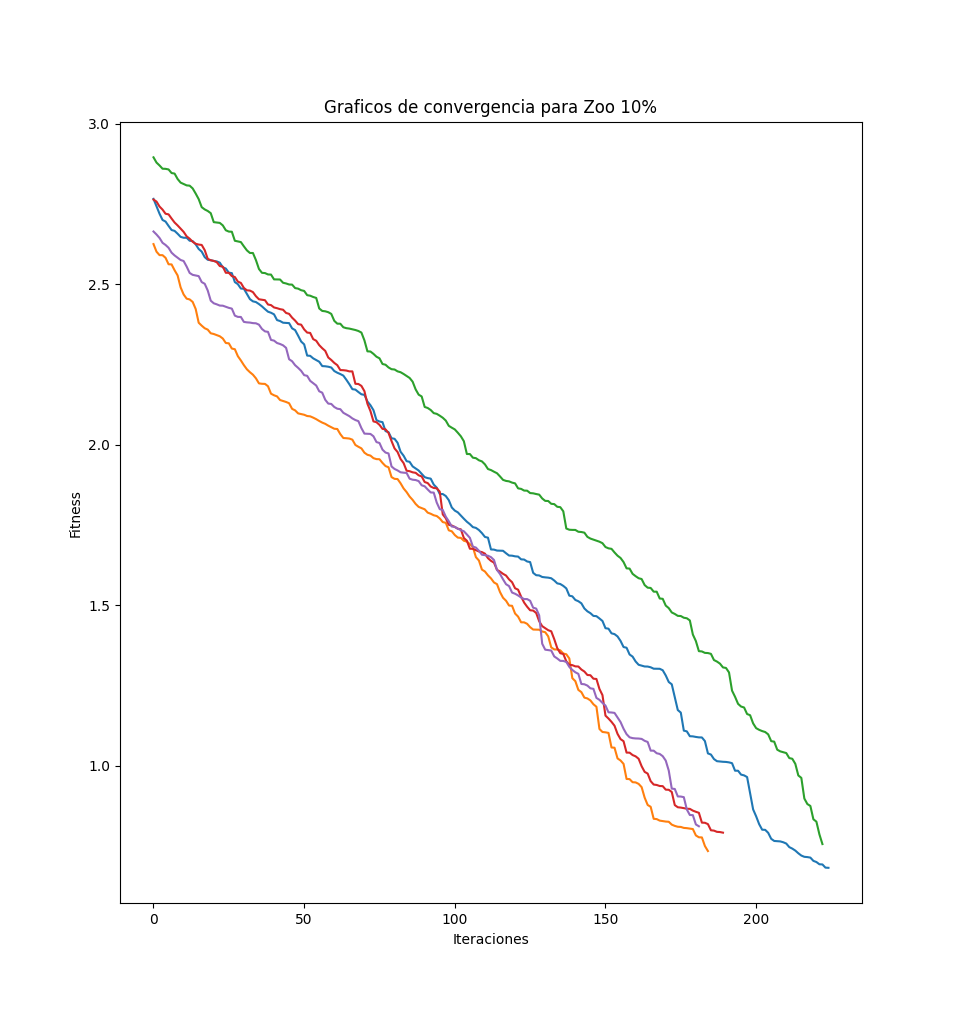
\includegraphics[scale=0.5]{convergencia_zoo_10}

Con esta gráfica queda claro el impacto que tiene la semilla inicial, tanto para la calidad de la solución obtenida, como para el número de iteraciones necesarias para conseguir alcanzar un óptimo local. Podemos mostrar la misma gráfica para Bupa 20\%:

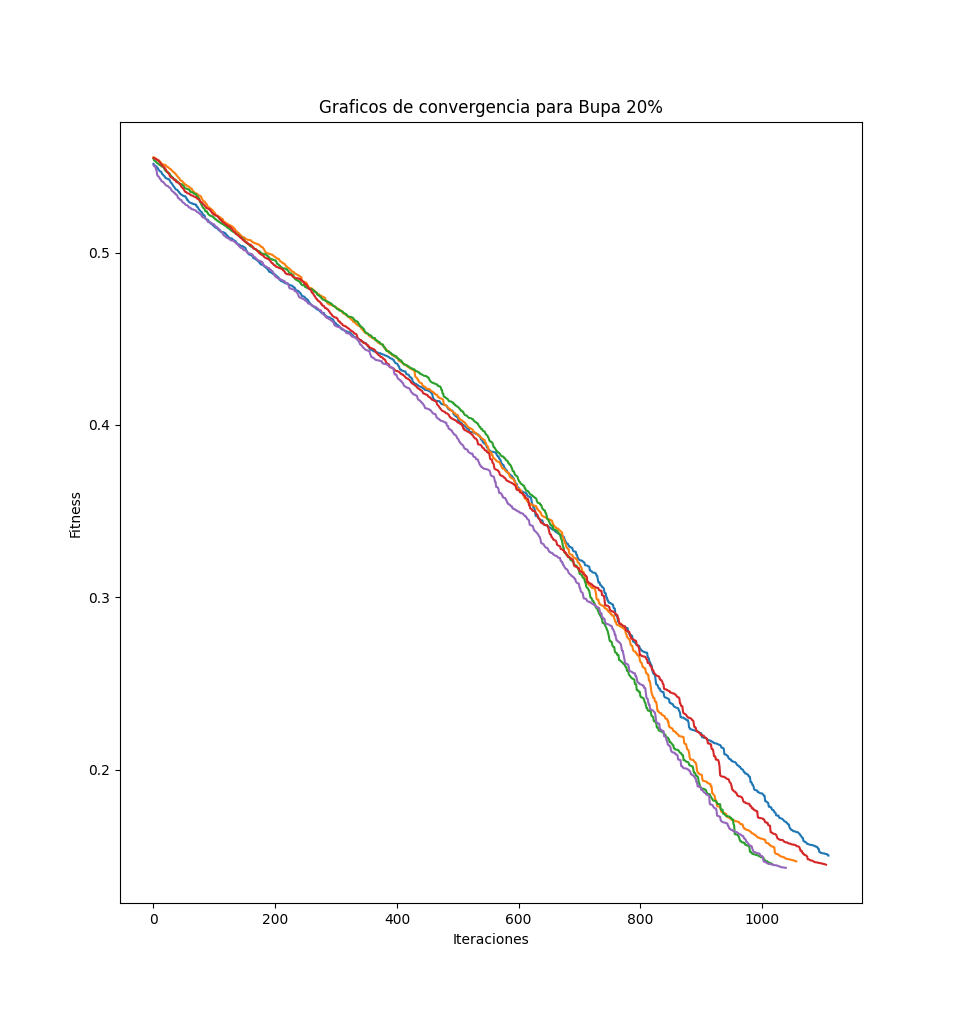
\includegraphics[scale=0.5]{convergencia_bupa_20}

Esta gráfica refuerza de nuevo todo lo que venimos desarrollando en relación a la influencia de la semilla aleatoria. Ambas gráficas también dejan claro que la evolución del fitness es estrictamente decreciente. Esto pues estamos haciendo una búsqueda el primero mejor, por tanto, siempre nos movemos hacia soluciones de mejor fitness.

\subsubsection{Posibles mejoras}

Para comenzar, sería interesante realizar un estudio sobre el valor de $\lambda$, buscando métodos o valores para que produzca soluciones con un mejor valor del $fitness$. En segundo lugar, hemos visto la sensibilidad de la búsqueda local a la semilla aleatoria. Esto puede movitar el interés por otros métodos como el de realizar búsquedas múltiples partiendo de distintas soluciones iniciales.

\pagebreak

\section{Bibliografía}

\bibliography{References}
\bibliographystyle{ieeetr}

\end{document}
